% !TeX spellcheck = pl_PL
\section{System przechowywania \newline danych}
Rozdział ten przedstawia propozycję systemu przechowywania danych. Struktura sieci informatycznej jest rozbudowana, zatem aby scentralizować dostęp do danych zastosowano technologię NAS. 

\subsection{Struktura NAS}
Dostęp do serwera NAS nie wymagają telefony IP oraz bramka VoIP, zatem nie zostały uwzględnione w strukturze. Schemat systemu NAS znajduje się na rysunku \ref{schemat:schemat_sieci_NAS}. Połączenia pomiędzy stacjami roboczymi poprowadzone są poprzez iSCSI (wykorzystując sieć przewodową).
\begin{landscape}
	\hspace{4cm}
	\begin{figure}[!h]
		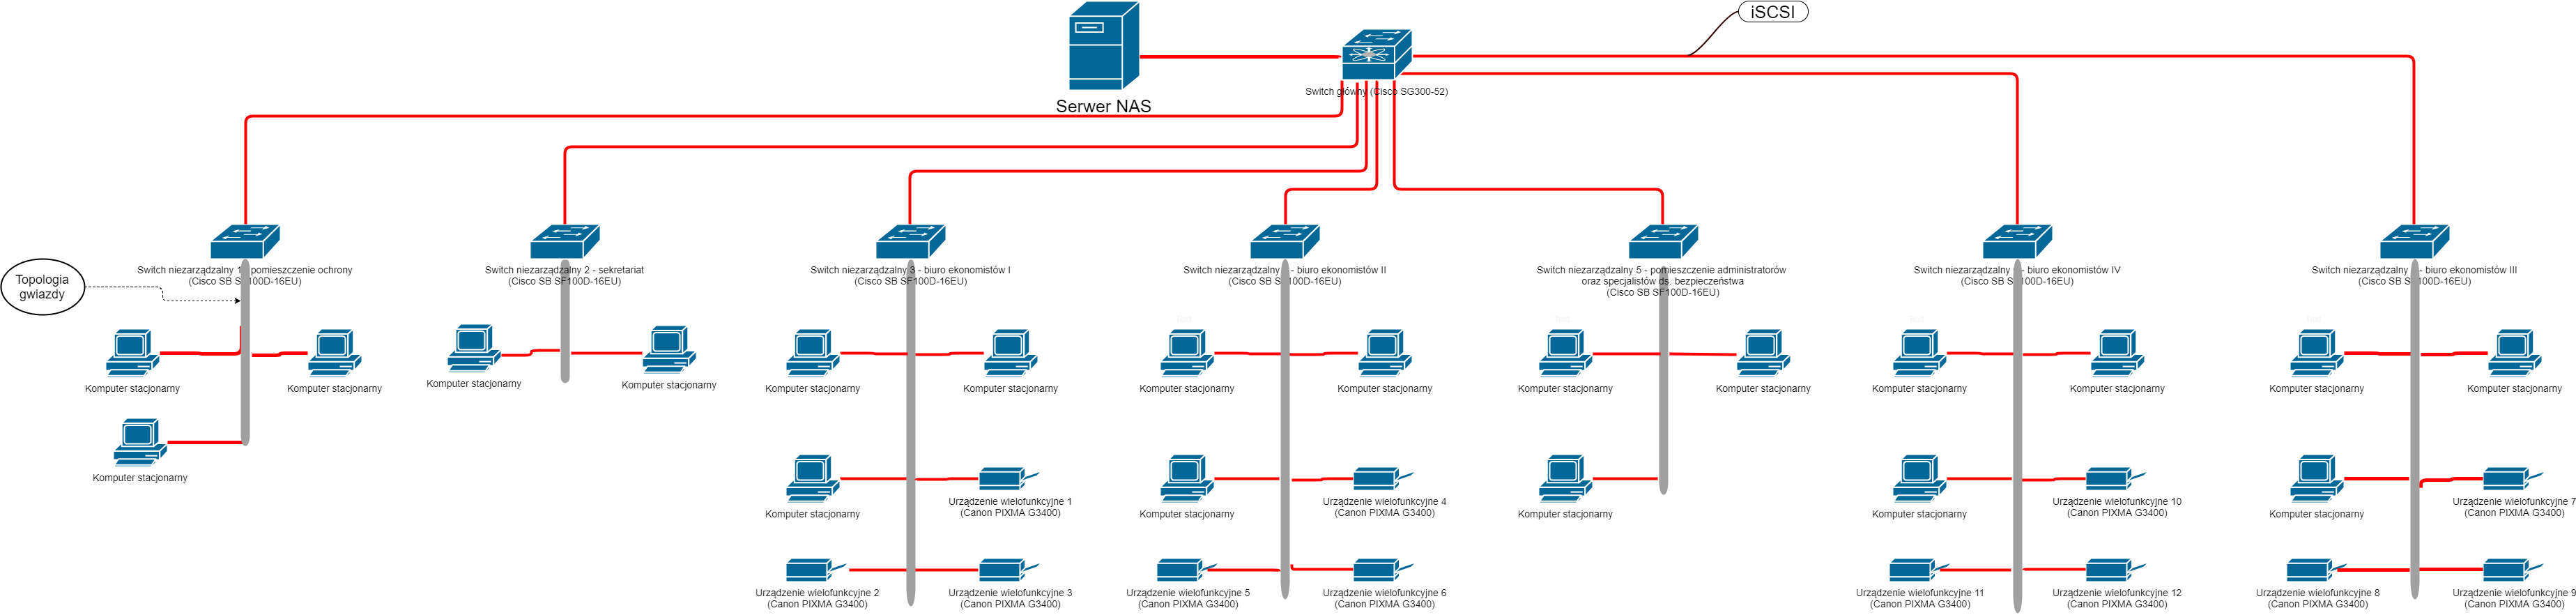
\includegraphics[width=24cm]{Schemat_NAS.png}
		\caption{Schemat struktury NAS}
		\label{schemat:schemat_sieci_NAS}
	\end{figure}
\end{landscape}

\subsection{Serwer}
Serwer główny ze względu na potrzebę niezawodności pracy posiada macierz dyskową RAID 4 z 3 dyskami HDD każdy o pojemności 2TB. W przypadku awarii dowolnego dysku istnieje możliwość odtworzenia utraconych danych. Jest to wolniejsze rozwiązanie niż powiedzmy RAID 5, ale zapewnia większe bezpieczeństwo w przypadku uszkodzenia. Wykorzystując daną macierz dyskową posiadamy 4TB pojemności dyskowej, wg podanych informacji od zleceniodawców taki rozmiar pamięci powinien wystarczyć na przechowywanie danych przez 50 lat (jest to okres przez jaki należy przechowywać dane księgowe).

Serwer zapasowy posiada kompletną kopię macierzy dyskowej z serwera głównego zapewniając redundancję w przypadku całkowitej awarii sprzętu. W~ten sposób zabezpieczamy w znacznym stopniu dane przed utraceniem.

Na serwerze w środowisku wirtualnym uruchomiony jest system FreeNAS odpowiedzialny za zarządzanie przechowywaniem plików. W systemie FreeNAS uruchomione są usługi odpowiedzialne za replikację danych oraz tworzenie kopii zapasowych. W razie potrzeby można zainstalować wtyczkę obsługującą własną chmurę ''Owncloud''.

Dodatkowo kopie zapasowe z okresu powyżej roku przechowywane są na taśmach magnetycznych w pomieszczeniu archiwum.

\subsection{Komputery pracowników}
Komputery pracowników ze względu na nie zbyt wysoką szkodliwość utraty danych (pod warunkiem przenoszenia danych systematycznie do pamięci serwera - NAS) nie wymagają szczególnych zabezpieczeń. Wykorzystano dwa rodzaje dysków: HDD (500GB) dla plików oraz SSD(120GB) dla wybranych programów oraz systemu operacyjnego. W przypadku braku dwóch slotów dyskowych drugi dysk (HDD) zastępuje napęd optyczny. Magistralą użytą w komputerach jest SATAIII ze względu na parametry techniczne komputerów (brak magistrali NVIe).